\chapter{Telematik}

Zusammenfassung der Vorlesung "`Telematik"' aus dem Wintersemester 2016.\footnote{\url{https://telematics.tm.kit.edu/ws201617_telematik.php}}

\section{Transportprotokolle}

\subsection{GrundlegendeKomponenten}

\subsubsection{TCP-Grundlagen}
\begin{itemize}
	\item \textbf{TCP-Verbindungsverwaltung}
	\begin{itemize}
		\item Identifikation einer TCP-Verbindung: Quell-/Zieladresse sowie Quell-/Zielport
		\item Verbindungsaufbau: Server wartet, Client initiiert Verbindung
		\item 3-Wege-Handshake
		\begin{enumerate}
			\item Client \(\rightarrow\) Server: \texttt{TConReq(SYN=1,seq=client\_isn)}
			\item Client \(\leftarrow\) Server: \texttt{TConCnf(SYN=1,ACK=1,seq=server\_isn,ack=client\_isn+1)}
			\item Client \(\rightarrow\) Server: \texttt{ACK(SYN=0,ACK=1,seq=client\_isn+1,ack=server\_isn+1)}
		\end{enumerate}
		\item Zusätzlich: Festlegen der initialen Sequenznummer (\texttt{isn}), Bekanntgabe der Größe des Flusskontrollfensters, Allokation der Puffer
		\item Format einer TCP-Dateneinheit\footnote{\url{https://upload.wikimedia.org/wikipedia/de/f/fd/TCP_Header.svg}}\\
			\begin{minipage}{\linewidth}
				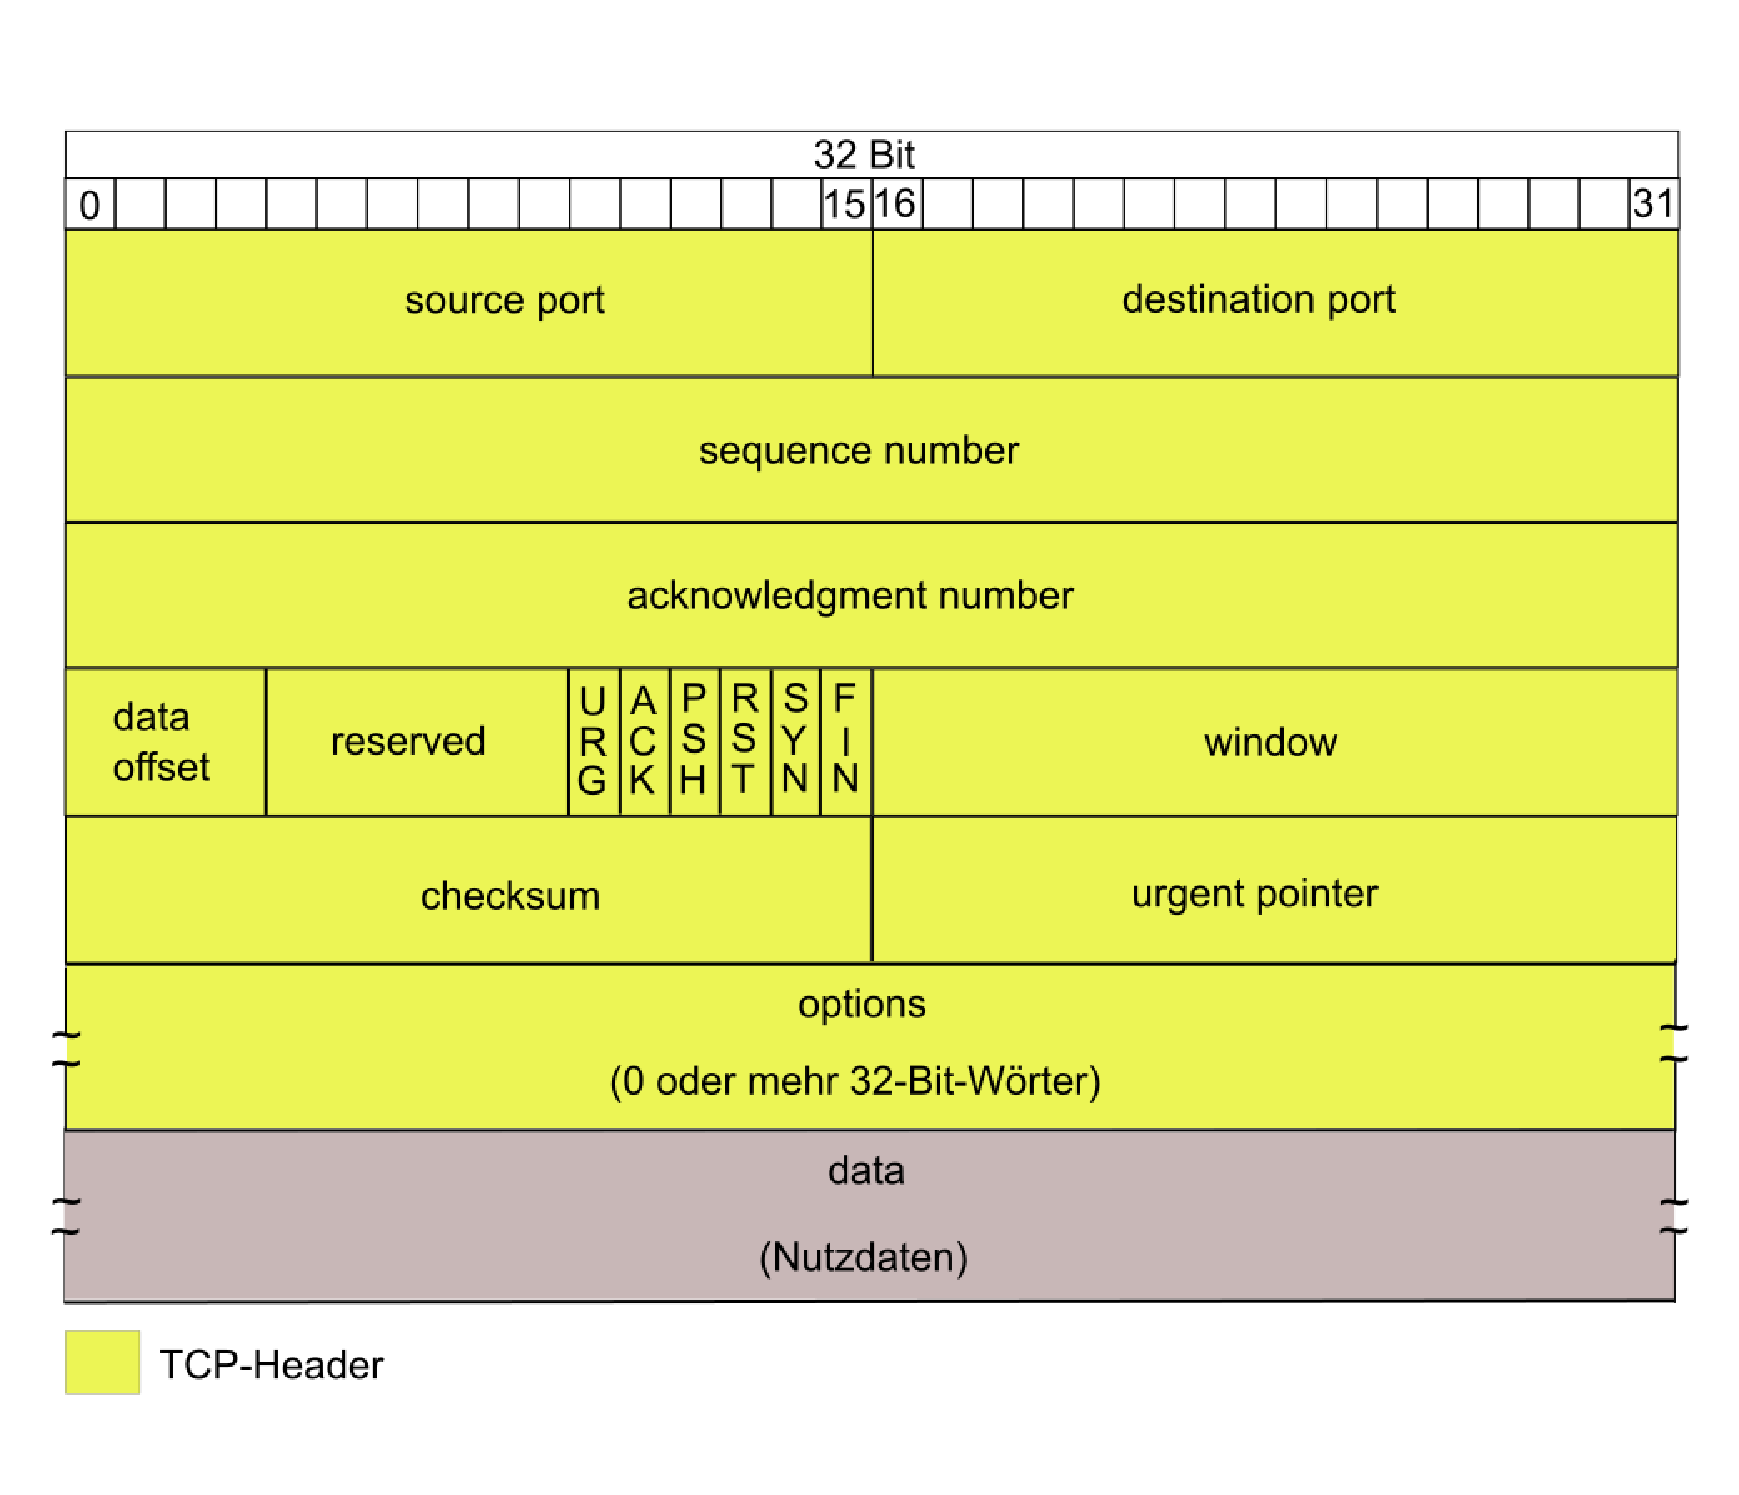
\includegraphics[scale=0.38]{telematik/TCP_Header.pdf}
			\end{minipage}
	\end{itemize}
	\item \textbf{Flusskontrolle zur Schutz des Empfängers vor zu hoher Last}
	\begin{itemize}
		\item Dynamische Anpassung des Empfangsfenster auf Empfängerseite, um die aktuelle verfügbare Puffergröße mitzuteilen. \texttt{RcvWindow} bezeichnet den Anteil des \texttt{RecvBuffer}, das frei ist (jeweils absolute Werte)
		\item Problem: \textit{Zero Window Probing}. Empfänger meldet ein volles Empfangsfenster. Wie weis der Sender, ab wann er wieder senden darf? Empfänger muss daher auch bei vollem Empfangsfenster Dateneinheiten mit einem Byte Länge quittieren
	\end{itemize}
	\item \textbf{Angriffe auf den Verbindungsaufbau: SYN-Flooding}
	\begin{itemize}
		\item Massenhaftes Senden von SYN-Dateneinheiten ohne Verbindungsaufbau. Problem: Zustandshaltung auf Empfängerseite für halboffene Verbindungen. Folge: Ressourcen erschöpft, Empfänger kann keine Dateneinheiten mehr annehmen
		\item Lösung: SYN-Cookies
		\begin{itemize}
			\item Verhinderung der Zustandshaltung bis zum letztmöglichen Zeitpunkt: Beginn der Zustandhaltung erst bei Empfang des \texttt{ACK}
			\item Realisierung: Ermittlung der Zustandsinformationen auf Empfängerseite anhand der Informationen aus \texttt{ACK(SYN=0,ACK=1,seq=client\_isn+1,ack=server\_isn+1)}
			\item Kodierungsbeispiel: Zeitstempel zur Verhinderung von Replay-Attacken (5 Bit); ausgewählte MSS aus acht vordefinierten Werten (3 Bit); Hash über Quelladresse und -port sowie Zieladresse und -port, verifiziert dass der Client bereits \texttt{SYN} durchgeführt hat /24 Bit). Daraus entsteht die 32 Bit initiale Sequenznummer des Servers
			\item Nachteil: Vergleichsweise kurze Sequenznummer reicht nicht für zusätzliche TCP-Optionen und limitiert MSS-Größen auf vordefinierte Werte
			\item Idee: Cookie erst einsetzen, wenn nötig (volle Warteschlange oder Ressourcenengpass)
		\end{itemize}
	\end{itemize}
\end{itemize}

\subsubsection{Staukontrolle}
\begin{itemize}
	\item Beobachtung: Unverhältnismäßiger Leistungseinbruch an Engstellen bei großem Datenaufkommen zwischen zwei schnelleren Netzen \(\rightarrow\) Warteschlangenmanagement notwendig
	\item \textbf{Einfaches Warteschlangenmanagement}
	\begin{itemize}
		\item Puffer im Router voll, nächste Dateneinheit muss verworfen werden ("`Tail Drop"'
		')
		\item Retransmissiontimer im Client steuert Sendewiederholungen
		\item Problem: Synchronisation. Dateineinheiten von mehreren Verbindungen werden quasi gleichzeitig verworfen
	\end{itemize}
	\item \textbf{Aktives Warteschlangenmanagement}
	\begin{itemize}
		\item Das Netz gibt einen Hinweis auf eine entstehende Stausituation
		\item Router verwirft (randomisiert) Dateneinheiten, bevor die Warteschlange voll ist
		\item Verfahren
		\begin{itemize}
			\item Konkrete Implementierung: Random Early Detection (RED)
			\begin{itemize}
				\item Wahrscheinlichkeit, dass eine Dateneinheit verworfen wird, steigt linear mit der Warteschlangenlänge
			\end{itemize}
		\end{itemize}
	\end{itemize}
	\item \textbf{Self-Clocking}
	\begin{itemize}
		\item Szenario: Verbindung zweier Netze über langsames Weitverkehrsnetz. Dateneinheiten benötigen bei der langsamen Übertragung mehr Zeit als in den lokalen Netzen. Dadurch kommen sie verzögert beim Empfänger an, welcher sie entsprechend "`langsam"' quittiert. Durch den entstehenden Takt weis der Sender, wie schnell er senden kann. Aber: Wie soll die "`Uhr"' gestartet werden
		\item Wieso wird kein Gleichgewicht erreicht?
		\begin{itemize}
			\item Verbindung kommt nicht ins Gleichgewicht
			\item Sender sendet neue Dateneinheiten zu früh
			\item Ressourcenbeschränkungen verhindern Gleichgewicht
		\end{itemize}
	\end{itemize}
\end{itemize}


\subsection{Analyse und Randbedingungen}


\subsection{Aktuelle Entwicklungen}
